\section{Power switching circuit}

Sự sập nguồn điện chính có thể rất quan trọng trong nhiều tình huống khác nhau. Ví dụ, khi nguồn điện bị mất đột ngột, bạn có thể muốn lưu một số dữ liệu dự phòng trên vi điều khiển. Những trường hợp như vậy cần một số mạch chuyển đổi tự động sang nguồn điện dự phòng, chẳng hạn như pin.

\begin{figure}[H]
    \centering
    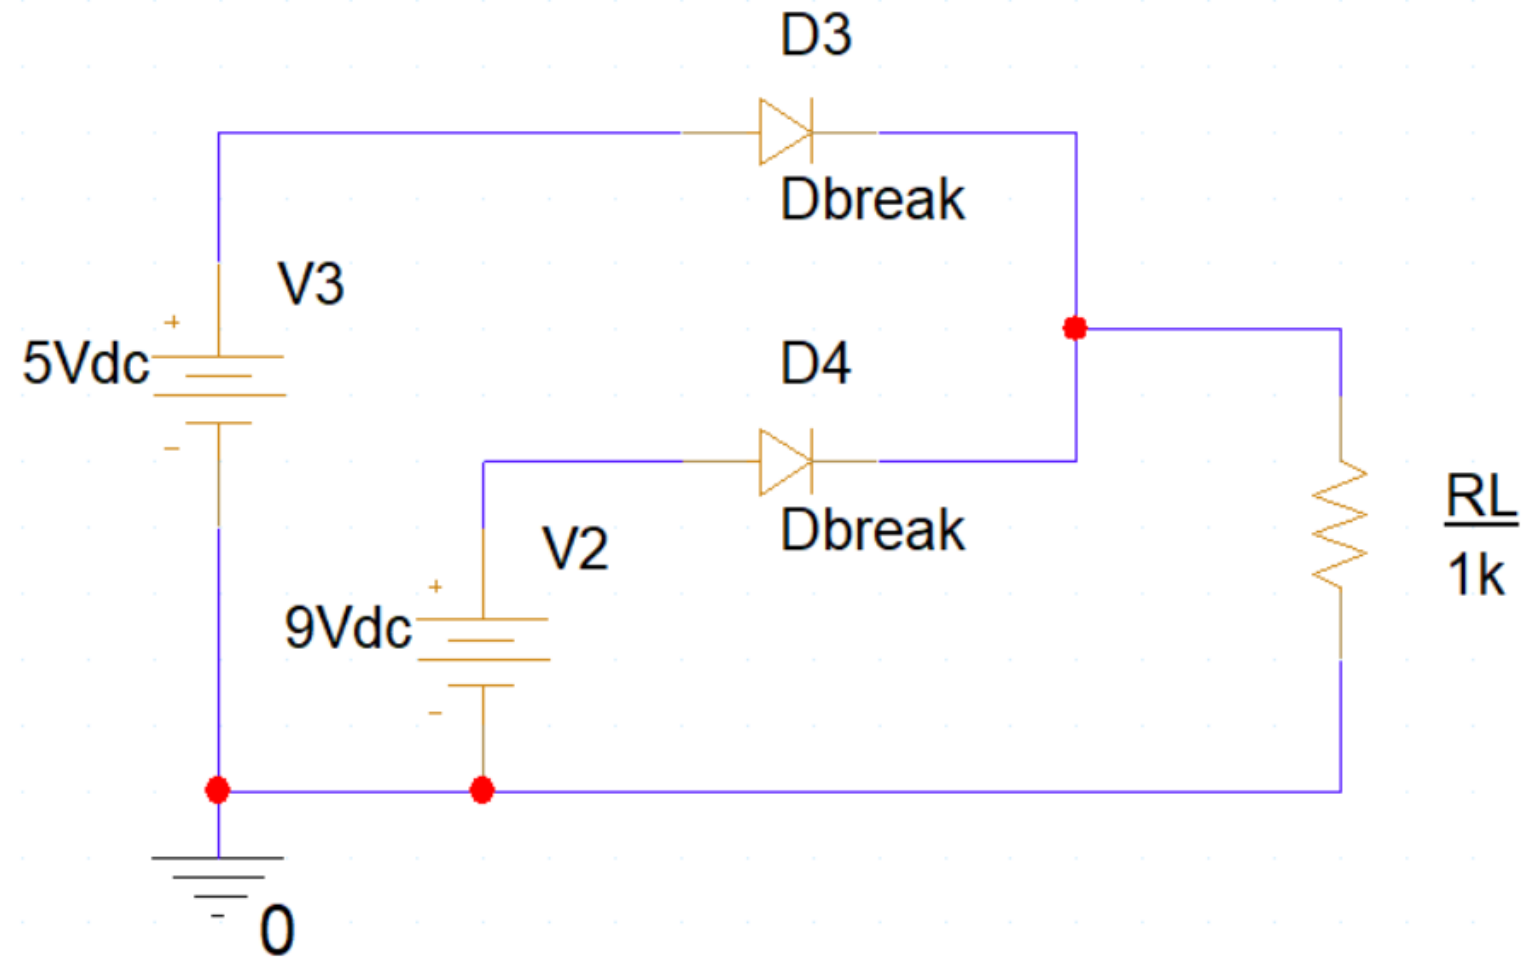
\includegraphics[width=0.8\textwidth]{graphics/ex5/f1.png}
    \caption{Mạch chuyển nguồn điện}
\end{figure}
Giải pháp đơn giản nhất cho vấn đề này là thêm một diode vào mỗi nguồn điện, như được hiển thị trong hình trên. Trong mạch này, nguồn điện 5V được sử dụng là một pin dự phòng. Trong khi đó, 9V là nguồn điện chính cho hệ thống, được minh họa bằng một điện trở tải.


Tuy nhiên, vấn đề của cách tiếp cận có phần ngây thơ này là sự sụt áp (phân cực thuận) qua diode có thể quá cao đối với hệ thống. Nhờ vào diode Schottky, điều này có thể được giảm thiểu bằng cách sử dụng loại có điện áp thuận cực thấp, có thể tìm thấy trên thị trường (ví dụ: diode Schottky sụt áp khoảng 250mV tại 1A).

\subsection{Tính toán theo lý thuyết}
\subsubsection{Trường hợp chỉ có nguồn 5V}
Dễ thấy D4 là diode phân cực nghịch nên không dẫn điện. Do đó, \(I_{D4} = 0\). Các đại lượng còn lại được tính như sau:
\begin{align*}
I_{D3} &= \frac{5V - V_{D3}}{R_{L}} = \frac{5V - 0.7V}{1k\Omega} = 4.3mA  \\
% I_{D4} &= 0 \\
I_{RL} &= I_{D3} = 4.3mA \\
V_{RL} &= I_{RL} \times R_{L} = 4.3mA \times 1k\Omega = 4.3V
\end{align*}

\subsubsection{Trường hợp chỉ có nguồn 9V}
Dễ thấy D3 là diode phân cực nghịch nên không dẫn điện. Do đó, \(I_{D3} = 0\). Các đại lượng còn lại được tính như sau:
\begin{align*}
% I_{D3} &= 0 \\
I_{D4} &= \frac{9V - V_{D4}}{R_{L}} = \frac{9V - 0.7V}{1k\Omega} = 8.3mA\\
I_{RL} &= I_{D4} = 8.3mA \\
V_{RL} &= I_{RL} \times R_{L} = 8.3mA \times 1k\Omega = 8.3V
\end{align*}

\subsubsection{Trường hợp có cả nguồn 5V và nguồn 9V}
Trường hợp này ta thấy D4 là diode phân cực thuận, D3 là diode phân cực nghịch nên không dẫn điện, \(I_{3} = 0V\). Các đại lượng còn lại được tính như sau:
\begin{align*}
% I_{D3} &= \frac{5V - V_{D3}}{R_{L}} \\
I_{D4} &= \frac{9V - V_{D4}}{R_{L}} = \frac{9V - 0.7V}{1k\Omega} = 8.3mA\\
I_{RL} &= I_{D4} = 8.3mA \\
V_{RL} &= I_{RL} \times R_{L} = 8.3mA \times 1k\Omega = 8.3V
\end{align*}

\subsection{Mô phỏng PSpice}
\begin{figure}[H]
    \centering
    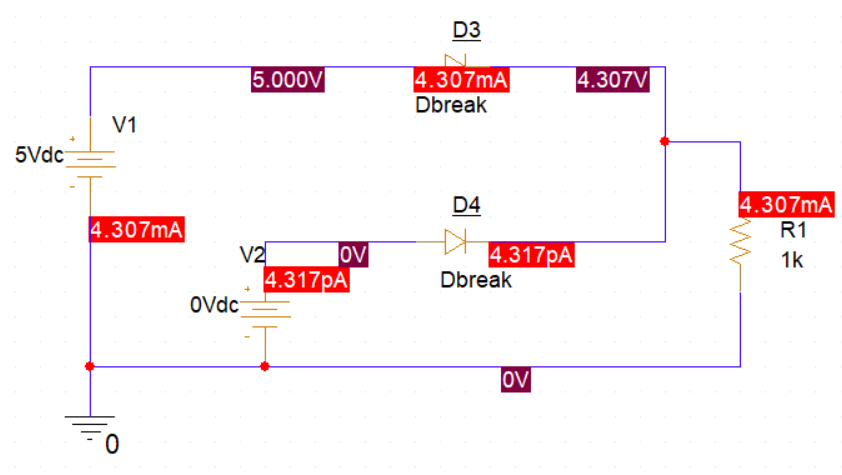
\includegraphics[width=1\textwidth]{graphics/ex5/f2.png}
    \caption{Trường hợp chỉ có nguồn 5V}
\end{figure}

\begin{figure}[H]
    \centering
    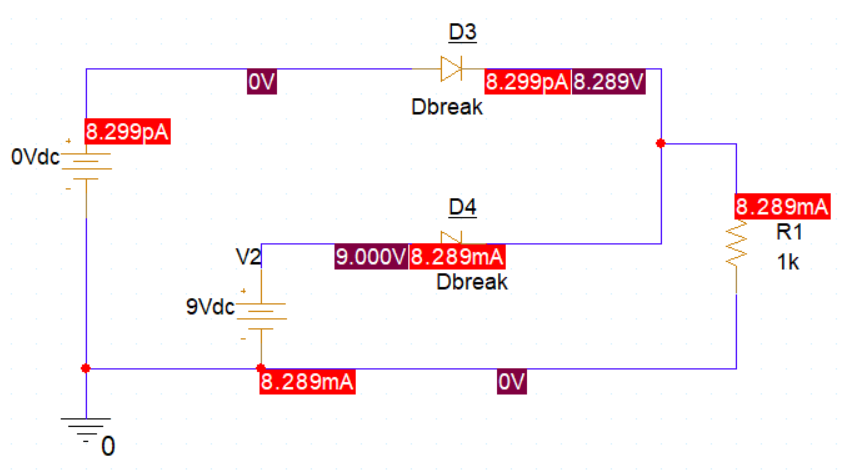
\includegraphics[width=1\textwidth]{graphics/ex5/f3.png}
    \caption{Trường hợp chỉ có nguồn 9V}
\end{figure}

\begin{figure}[H]
    \centering
    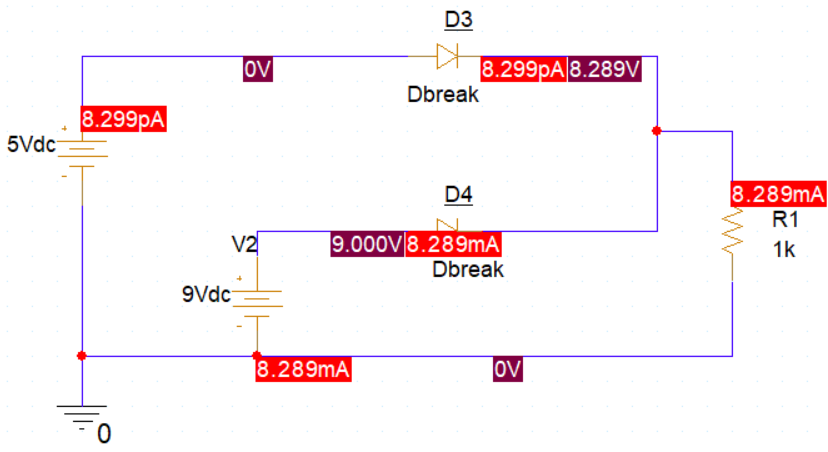
\includegraphics[width=1\textwidth]{graphics/ex5/f4.png}
    \caption{Trường hợp có cả nguồn 5V và nguồn 9V}
\end{figure}

\subsection{So sánh}
\begin{table}[H]
    \centering
    \begin{tabular}{|c|c|c|c|c|c|c|c|c|}
        \cline{2-9}
        \multicolumn{1}{c|}{} & \multicolumn{4}{c|}{\textbf{Tính toán theo lý thuyết}} & \multicolumn{4}{c|}{\textbf{Mô phỏng PSpice}} \\ \cline{2-9}
        \multicolumn{1}{c|}{} & \(I_{D3}\) & \(I_{D4}\) & \(I_{RL}\) & \(V_{RL}\) & \(I_{D3}\) & \(I_{D4}\) & \(I_{RL}\) & \(V_{RL}\) \\ \hline
        \textbf{Chỉ 5V} & 4.3mA & 0A & 4.3mA & 4.3V & 4.307mA & 4.317pA & 4.307mA & 4.307V \\ \hline
        \textbf{Chỉ 9V} & 0A & 8.3mA & 8.3mA & 8.3V & 8.299pA & 8.289mA & 8.289mA & 8.289V \\ \hline
        \textbf{5V và 9V} & 0A & 8.3mA & 8.3A & 8.3V & 8.299pA & 8.289mA & 8.289mA & 8.289V \\ \hline
    \end{tabular}
\end{table}

Chức năng cuối cùng của các diode trong mạch này là bảo vệ mạch khỏi dòng điện ngược chiều trong trường hợp cả hai nguồn được bật cùng lúc. Trường hợp này rất phổ biến khi vi điều khiển được lập trình và cấp nguồn bởi đồng thời cổng USB và nguồn điện bên ngoài.